% UTF-8 encoding
% Compile with latex+dvipdfmx, pdflatex, xelatex or lualatex
% XeLaTeX is recommanded
\documentclass{article}
\usepackage[UTF8]{ctex}
\usepackage{booktabs}
\usepackage{fancyhdr}
\usepackage{float}
\usepackage{graphicx}
\usepackage{helvet}
\usepackage{hyperref}
\usepackage{tabularx}
\usepackage{xcolor}

\usepackage{listings}
\usepackage{tikz}

\usepackage{makeidx}         % allows index generation
\makeindex

\lstset{frame=tblr,
  rulecolor=\color{lightgray},
  language=Java,
  aboveskip=5mm,
  belowskip=5mm,
  showstringspaces=false,
  columns=flexible,
  basicstyle=\linespread{1.0}\small\ttfamily,
  numbers=none,
  % numberstyle=\tiny\color{gray},
  % keywordstyle=\color{blue},
  % commentstyle=\color{dkgreen},
  % stringstyle=\color{mauve},
  breaklines=true,
  breakatwhitespace=true,
  tabsize=3
}

\usepackage{framed}     % These needed for the code formatter
\usepackage{color}
\usepackage{fancyvrb}

% Use helvetica (sans) by default
\renewcommand{\familydefault}{\sfdefault}

% Greenish links
\hypersetup{
  colorlinks=true,
  linkcolor=blue!50!red,
  urlcolor=blue!50!red
}

\newcommand{\two}{\raise0.5ex\hbox{\footnotesize{2}}}

\newcommand{\iic}{I\two{}C}
\newcommand{\iicdriver}{I\two{}CDriver}
\newcommand{\degc}{$^{\circ}$C}

\setlength{\headheight}{40pt}
\setlength{\headsep}{0.2in}

\pagestyle{fancy}
\lhead{
\includegraphics[width=0.2\textwidth]{img/logo}}
\chead{\iicdriver{} User Guide}
\rhead{\thepage}
\cfoot{\textcopyright \the\year \ \ Excamera Labs}
\renewcommand{\headrulewidth}{0.5pt}
\renewcommand{\footrulewidth}{0.5pt}

\usepackage{array}
\newcolumntype{L}[1]{>{\raggedright\let\newline\\\arraybackslash\hspace{0pt}}m{#1}}
\newcolumntype{C}[1]{>{\centering\let\newline\\\arraybackslash\hspace{0pt}}m{#1}}
\newcolumntype{R}[1]{>{\raggedleft\let\newline\\\arraybackslash\hspace{0pt}}m{#1}}

\usepackage{setspace}

\newcommand{\heavyline}{\specialrule{1pt}{1pt}{1pt}}
\newcommand{\png}[1]{
\begin{figure}[H]
\begin{center}
\includegraphics[width=0.75\textwidth]{#1}
\end{center}
\end{figure}
}
\newcommand{\pngw}[2]{
\begin{figure}[H]
\begin{center}
\includegraphics[width=#2\textwidth]{#1}
\end{center}
\end{figure}
}

\usepackage{sphinx}

\newcommand{\mach}[1]{\texttt{\textbf{#1}}}
\newcommand{\gap}{\vspace{10pt}}

\newcommand\encircle[1]{%
  \tikz[baseline=(X.base)] 
   \node (X) [draw, shape=circle, inner sep=0] {\strut #1};}


\makeatletter
\def\PY@reset{\let\PY@it=\relax \let\PY@bf=\relax%
    \let\PY@ul=\relax \let\PY@tc=\relax%
    \let\PY@bc=\relax \let\PY@ff=\relax}
\def\PY@tok#1{\csname PY@tok@#1\endcsname}
\def\PY@toks#1+{\ifx\relax#1\empty\else%
    \PY@tok{#1}\expandafter\PY@toks\fi}
\def\PY@do#1{\PY@bc{\PY@tc{\PY@ul{%
    \PY@it{\PY@bf{\PY@ff{#1}}}}}}}
\def\PY#1#2{\PY@reset\PY@toks#1+\relax+\PY@do{#2}}

\expandafter\def\csname PY@tok@gd\endcsname{\def\PY@tc##1{\textcolor[rgb]{0.63,0.00,0.00}{##1}}}
\expandafter\def\csname PY@tok@gu\endcsname{\let\PY@bf=\textbf\def\PY@tc##1{\textcolor[rgb]{0.50,0.00,0.50}{##1}}}
\expandafter\def\csname PY@tok@gt\endcsname{\def\PY@tc##1{\textcolor[rgb]{0.00,0.27,0.87}{##1}}}
\expandafter\def\csname PY@tok@gs\endcsname{\let\PY@bf=\textbf}
\expandafter\def\csname PY@tok@gr\endcsname{\def\PY@tc##1{\textcolor[rgb]{1.00,0.00,0.00}{##1}}}
\expandafter\def\csname PY@tok@cm\endcsname{\let\PY@it=\textit\def\PY@tc##1{\textcolor[rgb]{0.25,0.50,0.50}{##1}}}
\expandafter\def\csname PY@tok@vg\endcsname{\def\PY@tc##1{\textcolor[rgb]{0.10,0.09,0.49}{##1}}}
\expandafter\def\csname PY@tok@m\endcsname{\def\PY@tc##1{\textcolor[rgb]{0.40,0.40,0.40}{##1}}}
\expandafter\def\csname PY@tok@mh\endcsname{\def\PY@tc##1{\textcolor[rgb]{0.40,0.40,0.40}{##1}}}
\expandafter\def\csname PY@tok@go\endcsname{\def\PY@tc##1{\textcolor[rgb]{0.53,0.53,0.53}{##1}}}
\expandafter\def\csname PY@tok@ge\endcsname{\let\PY@it=\textit}
\expandafter\def\csname PY@tok@vc\endcsname{\def\PY@tc##1{\textcolor[rgb]{0.10,0.09,0.49}{##1}}}
\expandafter\def\csname PY@tok@il\endcsname{\def\PY@tc##1{\textcolor[rgb]{0.40,0.40,0.40}{##1}}}
\expandafter\def\csname PY@tok@cs\endcsname{\let\PY@it=\textit\def\PY@tc##1{\textcolor[rgb]{0.25,0.50,0.50}{##1}}}
\expandafter\def\csname PY@tok@cp\endcsname{\def\PY@tc##1{\textcolor[rgb]{0.74,0.48,0.00}{##1}}}
\expandafter\def\csname PY@tok@gi\endcsname{\def\PY@tc##1{\textcolor[rgb]{0.00,0.63,0.00}{##1}}}
\expandafter\def\csname PY@tok@gh\endcsname{\let\PY@bf=\textbf\def\PY@tc##1{\textcolor[rgb]{0.00,0.00,0.50}{##1}}}
\expandafter\def\csname PY@tok@ni\endcsname{\let\PY@bf=\textbf\def\PY@tc##1{\textcolor[rgb]{0.60,0.60,0.60}{##1}}}
\expandafter\def\csname PY@tok@nl\endcsname{\def\PY@tc##1{\textcolor[rgb]{0.63,0.63,0.00}{##1}}}
\expandafter\def\csname PY@tok@nn\endcsname{\let\PY@bf=\textbf\def\PY@tc##1{\textcolor[rgb]{0.00,0.00,1.00}{##1}}}
\expandafter\def\csname PY@tok@no\endcsname{\def\PY@tc##1{\textcolor[rgb]{0.53,0.00,0.00}{##1}}}
\expandafter\def\csname PY@tok@na\endcsname{\def\PY@tc##1{\textcolor[rgb]{0.49,0.56,0.16}{##1}}}
\expandafter\def\csname PY@tok@nb\endcsname{\def\PY@tc##1{\textcolor[rgb]{0.00,0.50,0.00}{##1}}}
\expandafter\def\csname PY@tok@nc\endcsname{\let\PY@bf=\textbf\def\PY@tc##1{\textcolor[rgb]{0.00,0.00,1.00}{##1}}}
\expandafter\def\csname PY@tok@nd\endcsname{\def\PY@tc##1{\textcolor[rgb]{0.67,0.13,1.00}{##1}}}
\expandafter\def\csname PY@tok@ne\endcsname{\let\PY@bf=\textbf\def\PY@tc##1{\textcolor[rgb]{0.82,0.25,0.23}{##1}}}
\expandafter\def\csname PY@tok@nf\endcsname{\def\PY@tc##1{\textcolor[rgb]{0.00,0.00,1.00}{##1}}}
\expandafter\def\csname PY@tok@si\endcsname{\let\PY@bf=\textbf\def\PY@tc##1{\textcolor[rgb]{0.73,0.40,0.53}{##1}}}
\expandafter\def\csname PY@tok@s2\endcsname{\def\PY@tc##1{\textcolor[rgb]{0.73,0.13,0.13}{##1}}}
\expandafter\def\csname PY@tok@vi\endcsname{\def\PY@tc##1{\textcolor[rgb]{0.10,0.09,0.49}{##1}}}
\expandafter\def\csname PY@tok@nt\endcsname{\let\PY@bf=\textbf\def\PY@tc##1{\textcolor[rgb]{0.00,0.50,0.00}{##1}}}
\expandafter\def\csname PY@tok@nv\endcsname{\def\PY@tc##1{\textcolor[rgb]{0.10,0.09,0.49}{##1}}}
\expandafter\def\csname PY@tok@s1\endcsname{\def\PY@tc##1{\textcolor[rgb]{0.73,0.13,0.13}{##1}}}
\expandafter\def\csname PY@tok@sh\endcsname{\def\PY@tc##1{\textcolor[rgb]{0.73,0.13,0.13}{##1}}}
\expandafter\def\csname PY@tok@sc\endcsname{\def\PY@tc##1{\textcolor[rgb]{0.73,0.13,0.13}{##1}}}
\expandafter\def\csname PY@tok@sx\endcsname{\def\PY@tc##1{\textcolor[rgb]{0.00,0.50,0.00}{##1}}}
\expandafter\def\csname PY@tok@bp\endcsname{\def\PY@tc##1{\textcolor[rgb]{0.00,0.50,0.00}{##1}}}
\expandafter\def\csname PY@tok@c1\endcsname{\let\PY@it=\textit\def\PY@tc##1{\textcolor[rgb]{0.25,0.50,0.50}{##1}}}
\expandafter\def\csname PY@tok@kc\endcsname{\let\PY@bf=\textbf\def\PY@tc##1{\textcolor[rgb]{0.00,0.50,0.00}{##1}}}
\expandafter\def\csname PY@tok@c\endcsname{\let\PY@it=\textit\def\PY@tc##1{\textcolor[rgb]{0.25,0.50,0.50}{##1}}}
\expandafter\def\csname PY@tok@mf\endcsname{\def\PY@tc##1{\textcolor[rgb]{0.40,0.40,0.40}{##1}}}
\expandafter\def\csname PY@tok@err\endcsname{\def\PY@bc##1{\setlength{\fboxsep}{0pt}\fcolorbox[rgb]{1.00,0.00,0.00}{1,1,1}{\strut ##1}}}
\expandafter\def\csname PY@tok@kd\endcsname{\let\PY@bf=\textbf\def\PY@tc##1{\textcolor[rgb]{0.00,0.50,0.00}{##1}}}
\expandafter\def\csname PY@tok@ss\endcsname{\def\PY@tc##1{\textcolor[rgb]{0.10,0.09,0.49}{##1}}}
\expandafter\def\csname PY@tok@sr\endcsname{\def\PY@tc##1{\textcolor[rgb]{0.73,0.40,0.53}{##1}}}
\expandafter\def\csname PY@tok@mo\endcsname{\def\PY@tc##1{\textcolor[rgb]{0.40,0.40,0.40}{##1}}}
\expandafter\def\csname PY@tok@kn\endcsname{\let\PY@bf=\textbf\def\PY@tc##1{\textcolor[rgb]{0.00,0.50,0.00}{##1}}}
\expandafter\def\csname PY@tok@mi\endcsname{\def\PY@tc##1{\textcolor[rgb]{0.40,0.40,0.40}{##1}}}
\expandafter\def\csname PY@tok@gp\endcsname{\let\PY@bf=\textbf\def\PY@tc##1{\textcolor[rgb]{0.00,0.00,0.50}{##1}}}
\expandafter\def\csname PY@tok@o\endcsname{\def\PY@tc##1{\textcolor[rgb]{0.40,0.40,0.40}{##1}}}
\expandafter\def\csname PY@tok@kr\endcsname{\let\PY@bf=\textbf\def\PY@tc##1{\textcolor[rgb]{0.00,0.50,0.00}{##1}}}
\expandafter\def\csname PY@tok@s\endcsname{\def\PY@tc##1{\textcolor[rgb]{0.73,0.13,0.13}{##1}}}
\expandafter\def\csname PY@tok@kp\endcsname{\def\PY@tc##1{\textcolor[rgb]{0.00,0.50,0.00}{##1}}}
\expandafter\def\csname PY@tok@w\endcsname{\def\PY@tc##1{\textcolor[rgb]{0.73,0.73,0.73}{##1}}}
\expandafter\def\csname PY@tok@kt\endcsname{\def\PY@tc##1{\textcolor[rgb]{0.69,0.00,0.25}{##1}}}
\expandafter\def\csname PY@tok@ow\endcsname{\let\PY@bf=\textbf\def\PY@tc##1{\textcolor[rgb]{0.67,0.13,1.00}{##1}}}
\expandafter\def\csname PY@tok@sb\endcsname{\def\PY@tc##1{\textcolor[rgb]{0.73,0.13,0.13}{##1}}}
\expandafter\def\csname PY@tok@k\endcsname{\let\PY@bf=\textbf\def\PY@tc##1{\textcolor[rgb]{0.00,0.50,0.00}{##1}}}
\expandafter\def\csname PY@tok@se\endcsname{\let\PY@bf=\textbf\def\PY@tc##1{\textcolor[rgb]{0.73,0.40,0.13}{##1}}}
\expandafter\def\csname PY@tok@sd\endcsname{\let\PY@it=\textit\def\PY@tc##1{\textcolor[rgb]{0.73,0.13,0.13}{##1}}}

\def\PYZbs{\char`\\}
\def\PYZus{\char`\_}
\def\PYZob{\char`\{}
\def\PYZcb{\char`\}}
\def\PYZca{\char`\^}
\def\PYZam{\char`\&}
\def\PYZlt{\char`\<}
\def\PYZgt{\char`\>}
\def\PYZsh{\char`\#}
\def\PYZpc{\char`\%}
\def\PYZdl{\char`\$}
\def\PYZhy{\char`\-}
\def\PYZsq{\char`\'}
\def\PYZdq{\char`\"}
\def\PYZti{\char`\~}
% for compatibility with earlier versions
\def\PYZat{@}
\def\PYZlb{[}
\def\PYZrb{]}
\makeatother



\begin{document}

\newpage
\begin{center}
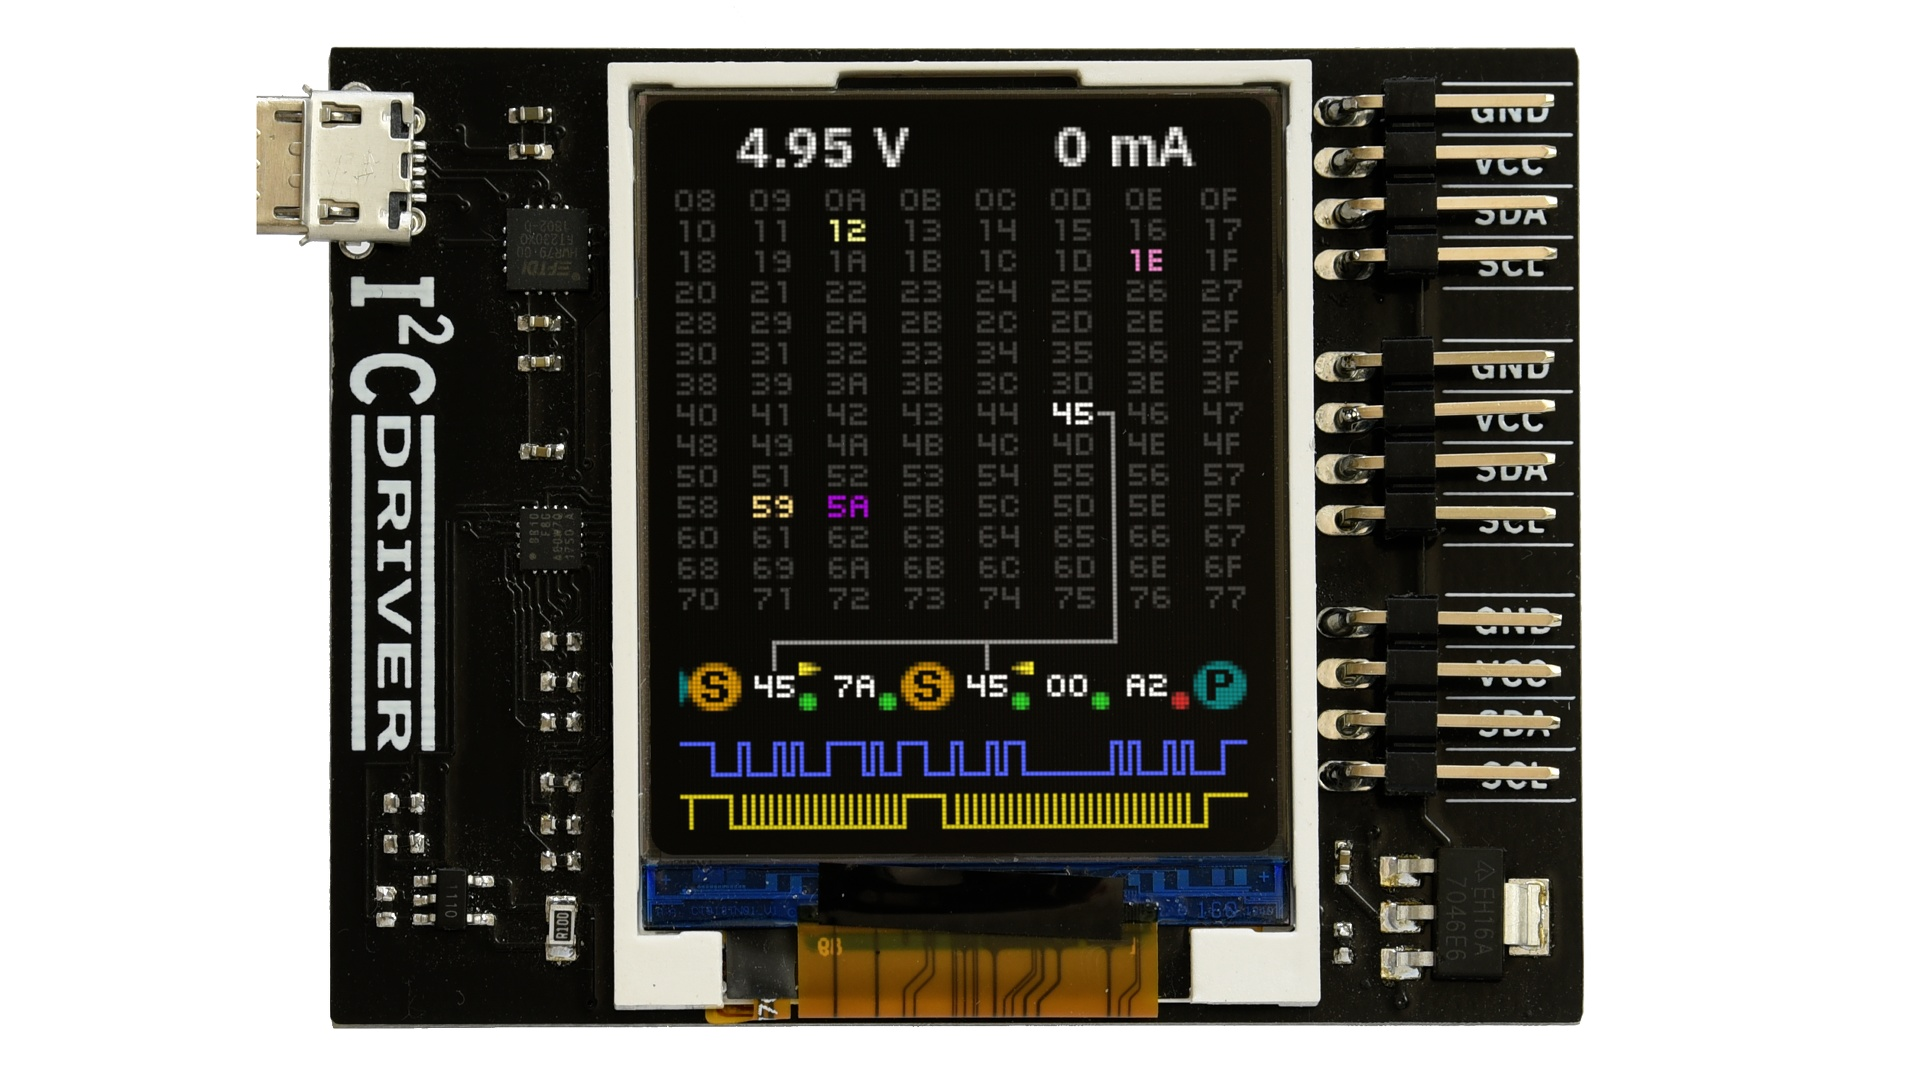
\includegraphics[width=1.00\textwidth]{img/i2cdriver/hero}
Last updated on \today
\end{center}
\tableofcontents

\newpage

\setlength{\parindent}{0mm}
\setlength{\parskip}{1mm}
\setstretch{1.4}

\section{概论}

\iicdriver{} 是一个易于使用,开源的工具,用于控制 \iic{} 设备. 它可以运行于 Windows, Mac, and Linux 平台上。 它内置彩色屏幕,可以实时显示所有的 \iic{} 活动信息. 由于使用标准的 FTDI USB 系列芯片 与计算机通讯,  所以不需要另外安装驱动程序.  它还包括了额外的3.3 V 电源, 方便用于监控电压和电流.

\subsection{特性}
\begin{itemize}
\item \textbf{实时显示}: 精确显示shows you exactly what it's doing all the time  
\item \textbf{支持所有 \iic{} 的特性}: 7- 和 10-比特 \iic{} 寻址, 时钟拉伸, 总线仲裁,400至100 KHz的传送速率
\item \textbf{\iic{} 上拉电阻}: 可编程 自动调整 \iic{}上拉电阻  
\item \textbf{USB 电压监控}: 侦测USB电压供应问题, 低至0.01v  
\item \textbf{目标设备电源监控}: 测量目标设备高侧电流, 精确至5 mA  
\item \textbf{三个 \iic{} 端口}: 三个完全相同的 \iic{} 端口, 各自有独立电源和 \iic{} 信号
\item \textbf{跳线}: 包括三组高质量彩色编码的100 毫米跳线
\item \textbf{3.3 V 输出}: 3.3 V 伏特  兼容5 伏特 
\item \textbf{高可靠性的组件}: 使用 FTDI USB 串口适配芯片, Silicon Labs 汽车级EFM8 控制器
\item \textbf{开源硬件}: 硬件设计, 固件和工具都在BSD 协议下开源 
\item \textbf{控制灵活}: 图形界面, 命令行, C/C++, Python 2/3 ,适用于 Windows, Mac, 和 Linux  
\end{itemize}

\newpage
\section{入门}

当你第一次连接 \iicdriver{}到USB 端口, 屏幕会闪烁白色后,显示如下:

\png{img/i2cdriver/DSC_9039}

连接三组不同颜色的跳线,按照如下的颜色标签:

\gap
\begin{center}
\begin{tabular}{ll}
\hline
\mach{GND}  & 黑色 \\
\mach{VCC}  & 红色 \\
\mach{SDA}  & 蓝色 \\
\mach{SCL}  & 黄色 \\
\hline
\end{tabular}
\end{center}
\gap

头两个信号分别传送3.3伏特电源 

在屏幕的顶端,\iicdriver{} 不间断的显示所测量的USB 总线电压和输出电流.

\newpage
\section{所需软件安装}

\iicdriver{} 软件源代码在
\href{https://github.com/jamesbowman/i2cdriver}{此处}.
包括:

\begin{itemize}
\item  Windows/Mac/Linux 图形工具
\item  Windows/Mac/Linux 命令行工具
\item Python 2 and 3 绑定库
\item C/C++ 绑定 (Windows/Mac/Linux)
\end{itemize}

安装图形和命令行工具会由因不同平台而有所差异.

\subsection{Windows}\index{drivers!Windows}

这里包含Windows下的图形和命令行工具
\href{https://i2cdriver.com/windows}{安装} .

图形界面的快捷方式安装在桌面上: 

\pngw{img/i2cdriver/win32-icon}{.3}

启动后会开启控制窗口:

\pngw{img/i2cdriver/win32-gui}{1.0}

若只有一个设备连接,则该\iicdriver{}设备被自动选择
若是超过一个设备, 在顶端的下拉菜单中选择对应COM 端口所连接的\iic{}设备
一旦建立连接, 你可以选择一个连接的设备并进行读写数据.

命令行工具 \mach{i2ccl}  已经被安装.  比如显示状态信息:

\begin{lstlisting}
c:\>"c:\Program Files\Excamera Labs\I2CDriver\i2ccl.exe" COM6 i
uptime 8991  4.957 V  30 mA  25.8 C SDA=1 SCL=1 speed=100 kHz
\end{lstlisting}

查看下面以获取更多命令行的用法.

\subsection{Linux}\index{drivers!Linux}

图形界面工具包含在\mach{i2cdriver} Python package, 同时兼容 Python 2 and 3.
若要安装, 打开一个shell prompt:

\begin{lstlisting}
sudo pip install i2cdriver
\end{lstlisting}

然后运行:

\begin{lstlisting}
i2cgui.py
\end{lstlisting}

使用命令行工具克隆\href{https://github.com/jamesbowman/i2cdriver}{I2CDriver 源码库},
然后:

\begin{lstlisting}
cd i2cdriver/c
make -f linux/Makefile
sudo make -f linux/Makefile install
i2ccl /dev/ttyUSB0 i
\end{lstlisting}

你会看到如下:

\begin{lstlisting}
uptime 1651  4.971 V  0 mA  21.2 C SDA=1 SCL=1 speed=100 kHz
\end{lstlisting}

\subsection{MacOS}\index{drivers!Mac}

图形界面工具包含在\mach{i2cdriver} Python package, 同时兼容 Python 2 and 3.
若要安装, 打开一个shell prompt:

\begin{lstlisting}
sudo pip install i2cdriver
\end{lstlisting}

Then run it with

\begin{lstlisting}
i2cgui.py
\end{lstlisting}


使用命令行工具, 克隆
\href{https://github.com/jamesbowman/i2cdriver}{I2CDriver 源码库},
然后:

\begin{lstlisting}
cd i2cdriver/c
make -f linux/Makefile
sudo make -f linux/Makefile install
i2ccl /dev/cu.usbserial-DO00QS8D i
\end{lstlisting}

(用你真实的 \iicdriver{}'s ID 来替换 \mach{DO00QS8D})
你会看到:

\begin{lstlisting}
uptime 1651  4.971 V  5 mA  21.2 C SDA=1 SCL=1 speed=100 kHz
\end{lstlisting}

请注意你所使用的端口是 \mach{/dev/cu.usbserial-XXXXXXXX}, 如
\href{https://pbxbook.com/other/mac-tty.html}{这里} 所解释的那样.

\newpage
\section{APIs}

\subsection{Python 2 和 3}\index{drivers!Python}

\iicdriver{} 绑定可以通过\mach{pip} 安装:

\begin{lstlisting}
  pip install i2cdriver
\end{lstlisting}

然后你就可以用Python读取 LM75B 温度传感器:
\index{Example!LM75B}

\begin{lstlisting}
>>> import i2cdriver
>>> i2c = i2cdriver.I2CDriver("/dev/ttyUSB0")
>>> d=i2cdriver.EDS.Temp(i2c)
>>> d.read()
17.875
>>> d.read()
18.0
\end{lstlisting}

你可以打印出总线信息,使用\index{bus scan}:

\begin{lstlisting}
>>> i2c.scan()
-- -- -- -- -- -- -- -- 
-- -- -- -- -- -- -- -- 
-- -- -- -- 1C -- -- -- 
-- -- -- -- -- -- -- -- 
-- -- -- -- -- -- -- -- 
-- -- -- -- -- -- -- -- 
-- -- -- -- -- -- -- -- 
-- -- -- -- -- -- -- -- 
48 -- -- -- -- -- -- -- 
-- -- -- -- -- -- -- -- 
-- -- -- -- -- -- -- -- 
-- -- -- -- -- -- -- -- 
68 -- -- -- -- -- -- -- 
-- -- -- -- -- -- -- -- 
[28, 72, 104]
\end{lstlisting}

Python 图形界面 (使用 \href{https://www.wxpython.org/pages/downloads/}{wxPython}) 可以这样启动:

\begin{lstlisting}
python i2cgui.py
\end{lstlisting}

根据你所安装的系统不同,会有:

\png{img/i2cdriver/win32-gui}

更多例子请参考:
\href{https://github.com/jamesbowman/i2cdriver/tree/master/python/samples}{samples folder in the repository}.

该模块带有丰富的帮助文档:
\begin{lstlisting}
>>> help(i2cdriver)
\end{lstlisting}
可以显示API文档.

\newpage
\subsubsection{参考}
\let\spxentry \sphinxstyleindexentry
\let\spxextra \sphinxstyleindexextra

\index{I2CDriver (class in i2cdriver)@\spxentry{I2CDriver}\spxextra{class in i2cdriver}}

\begin{fulllineitems}
\phantomsection\label{\detokenize{index:i2cdriver.I2CDriver}}\pysiglinewithargsret{\sphinxbfcode{\sphinxupquote{class }}\sphinxcode{\sphinxupquote{i2cdriver.}}\sphinxbfcode{\sphinxupquote{I2CDriver}}}{\emph{port='/dev/ttyUSB0'}, \emph{reset=True}}{}
A connected I2CDriver.
\begin{quote}\begin{description}
\item[{Variables}] \leavevmode\begin{itemize}
\item {} 
\sphinxstyleliteralstrong{\sphinxupquote{product}} \textendash{} product code e.g. ‘i2cdriver1’

\item {} 
\sphinxstyleliteralstrong{\sphinxupquote{serial}} \textendash{} serial string of I2CDriver

\item {} 
\sphinxstyleliteralstrong{\sphinxupquote{uptime}} \textendash{} time since I2CDriver boot, in seconds

\item {} 
\sphinxstyleliteralstrong{\sphinxupquote{voltage}} \textendash{} USB voltage, in V

\item {} 
\sphinxstyleliteralstrong{\sphinxupquote{current}} \textendash{} current used by attached device, in mA

\item {} 
\sphinxstyleliteralstrong{\sphinxupquote{temp}} \textendash{} temperature, in degrees C

\item {} 
\sphinxstyleliteralstrong{\sphinxupquote{scl}} \textendash{} state of SCL

\item {} 
\sphinxstyleliteralstrong{\sphinxupquote{sda}} \textendash{} state of SDA

\item {} 
\sphinxstyleliteralstrong{\sphinxupquote{speed}} \textendash{} current device speed in KHz (100 or 400)

\item {} 
\sphinxstyleliteralstrong{\sphinxupquote{mode}} \textendash{} IO mode (I2C or bitbang)

\item {} 
\sphinxstyleliteralstrong{\sphinxupquote{pullups}} \textendash{} programmable pullup enable pins

\item {} 
\sphinxstyleliteralstrong{\sphinxupquote{ccitt\_crc}} \textendash{} CCITT-16 CRC of all transmitted and received bytes

\end{itemize}

\end{description}\end{quote}
\index{\_\_init\_\_() (i2cdriver.I2CDriver method)@\spxentry{\_\_init\_\_()}\spxextra{i2cdriver.I2CDriver method}}

\begin{fulllineitems}
\phantomsection\label{\detokenize{index:i2cdriver.I2CDriver.__init__}}\pysiglinewithargsret{\sphinxbfcode{\sphinxupquote{\_\_init\_\_}}}{\emph{port='/dev/ttyUSB0'}, \emph{reset=True}}{}
Connect to a hardware i2cdriver.
\begin{quote}\begin{description}
\item[{Parameters}] \leavevmode\begin{itemize}
\item {} 
\sphinxstyleliteralstrong{\sphinxupquote{port}} (\sphinxhref{https://docs.python.org/3/library/stdtypes.html\#str}{\sphinxstyleliteralemphasis{\sphinxupquote{str}}}) \textendash{} The USB port to connect to

\item {} 
\sphinxstyleliteralstrong{\sphinxupquote{reset}} (\sphinxhref{https://docs.python.org/3/library/functions.html\#bool}{\sphinxstyleliteralemphasis{\sphinxupquote{bool}}}) \textendash{} Issue an I2C bus reset on connection

\end{itemize}

\end{description}\end{quote}

\end{fulllineitems}

\index{setspeed() (i2cdriver.I2CDriver method)@\spxentry{setspeed()}\spxextra{i2cdriver.I2CDriver method}}

\begin{fulllineitems}
\phantomsection\label{\detokenize{index:i2cdriver.I2CDriver.setspeed}}\pysiglinewithargsret{\sphinxbfcode{\sphinxupquote{setspeed}}}{\emph{s}}{}
Set the I2C bus speed.
\begin{quote}\begin{description}
\item[{Parameters}] \leavevmode
\sphinxstyleliteralstrong{\sphinxupquote{s}} (\sphinxhref{https://docs.python.org/3/library/functions.html\#int}{\sphinxstyleliteralemphasis{\sphinxupquote{int}}}) \textendash{} speed in KHz, either 100 or 400

\end{description}\end{quote}

\end{fulllineitems}

\index{setpullups() (i2cdriver.I2CDriver method)@\spxentry{setpullups()}\spxextra{i2cdriver.I2CDriver method}}

\begin{fulllineitems}
\phantomsection\label{\detokenize{index:i2cdriver.I2CDriver.setpullups}}\pysiglinewithargsret{\sphinxbfcode{\sphinxupquote{setpullups}}}{\emph{s}}{}
Set the I2CDriver pullup resistors
\begin{quote}\begin{description}
\item[{Parameters}] \leavevmode
\sphinxstyleliteralstrong{\sphinxupquote{s}} \textendash{} 6-bit pullup mask

\end{description}\end{quote}

\end{fulllineitems}

\index{scan() (i2cdriver.I2CDriver method)@\spxentry{scan()}\spxextra{i2cdriver.I2CDriver method}}

\begin{fulllineitems}
\phantomsection\label{\detokenize{index:i2cdriver.I2CDriver.scan}}\pysiglinewithargsret{\sphinxbfcode{\sphinxupquote{scan}}}{\emph{silent=False}}{}
Performs an I2C bus scan.
If silent is False, prints a map of devices.
Returns a list of the device addresses.

\begin{sphinxVerbatim}[commandchars=\\\{\}]
\PYG{g+gp}{\PYGZgt{}\PYGZgt{}\PYGZgt{} }\PYG{n}{i2c}\PYG{o}{.}\PYG{n}{scan}\PYG{p}{(}\PYG{p}{)}
\PYG{g+go}{\PYGZhy{}\PYGZhy{} \PYGZhy{}\PYGZhy{} \PYGZhy{}\PYGZhy{} \PYGZhy{}\PYGZhy{} \PYGZhy{}\PYGZhy{} \PYGZhy{}\PYGZhy{} \PYGZhy{}\PYGZhy{} \PYGZhy{}\PYGZhy{} }
\PYG{g+go}{\PYGZhy{}\PYGZhy{} \PYGZhy{}\PYGZhy{} \PYGZhy{}\PYGZhy{} \PYGZhy{}\PYGZhy{} \PYGZhy{}\PYGZhy{} \PYGZhy{}\PYGZhy{} \PYGZhy{}\PYGZhy{} \PYGZhy{}\PYGZhy{} }
\PYG{g+go}{\PYGZhy{}\PYGZhy{} \PYGZhy{}\PYGZhy{} \PYGZhy{}\PYGZhy{} \PYGZhy{}\PYGZhy{} 1C \PYGZhy{}\PYGZhy{} \PYGZhy{}\PYGZhy{} \PYGZhy{}\PYGZhy{} }
\PYG{g+go}{\PYGZhy{}\PYGZhy{} \PYGZhy{}\PYGZhy{} \PYGZhy{}\PYGZhy{} \PYGZhy{}\PYGZhy{} \PYGZhy{}\PYGZhy{} \PYGZhy{}\PYGZhy{} \PYGZhy{}\PYGZhy{} \PYGZhy{}\PYGZhy{} }
\PYG{g+go}{\PYGZhy{}\PYGZhy{} \PYGZhy{}\PYGZhy{} \PYGZhy{}\PYGZhy{} \PYGZhy{}\PYGZhy{} \PYGZhy{}\PYGZhy{} \PYGZhy{}\PYGZhy{} \PYGZhy{}\PYGZhy{} \PYGZhy{}\PYGZhy{} }
\PYG{g+go}{\PYGZhy{}\PYGZhy{} \PYGZhy{}\PYGZhy{} \PYGZhy{}\PYGZhy{} \PYGZhy{}\PYGZhy{} \PYGZhy{}\PYGZhy{} \PYGZhy{}\PYGZhy{} \PYGZhy{}\PYGZhy{} \PYGZhy{}\PYGZhy{} }
\PYG{g+go}{\PYGZhy{}\PYGZhy{} \PYGZhy{}\PYGZhy{} \PYGZhy{}\PYGZhy{} \PYGZhy{}\PYGZhy{} \PYGZhy{}\PYGZhy{} \PYGZhy{}\PYGZhy{} \PYGZhy{}\PYGZhy{} \PYGZhy{}\PYGZhy{} }
\PYG{g+go}{\PYGZhy{}\PYGZhy{} \PYGZhy{}\PYGZhy{} \PYGZhy{}\PYGZhy{} \PYGZhy{}\PYGZhy{} \PYGZhy{}\PYGZhy{} \PYGZhy{}\PYGZhy{} \PYGZhy{}\PYGZhy{} \PYGZhy{}\PYGZhy{} }
\PYG{g+go}{48 \PYGZhy{}\PYGZhy{} \PYGZhy{}\PYGZhy{} \PYGZhy{}\PYGZhy{} \PYGZhy{}\PYGZhy{} \PYGZhy{}\PYGZhy{} \PYGZhy{}\PYGZhy{} \PYGZhy{}\PYGZhy{} }
\PYG{g+go}{\PYGZhy{}\PYGZhy{} \PYGZhy{}\PYGZhy{} \PYGZhy{}\PYGZhy{} \PYGZhy{}\PYGZhy{} \PYGZhy{}\PYGZhy{} \PYGZhy{}\PYGZhy{} \PYGZhy{}\PYGZhy{} \PYGZhy{}\PYGZhy{} }
\PYG{g+go}{\PYGZhy{}\PYGZhy{} \PYGZhy{}\PYGZhy{} \PYGZhy{}\PYGZhy{} \PYGZhy{}\PYGZhy{} \PYGZhy{}\PYGZhy{} \PYGZhy{}\PYGZhy{} \PYGZhy{}\PYGZhy{} \PYGZhy{}\PYGZhy{} }
\PYG{g+go}{\PYGZhy{}\PYGZhy{} \PYGZhy{}\PYGZhy{} \PYGZhy{}\PYGZhy{} \PYGZhy{}\PYGZhy{} \PYGZhy{}\PYGZhy{} \PYGZhy{}\PYGZhy{} \PYGZhy{}\PYGZhy{} \PYGZhy{}\PYGZhy{} }
\PYG{g+go}{68 \PYGZhy{}\PYGZhy{} \PYGZhy{}\PYGZhy{} \PYGZhy{}\PYGZhy{} \PYGZhy{}\PYGZhy{} \PYGZhy{}\PYGZhy{} \PYGZhy{}\PYGZhy{} \PYGZhy{}\PYGZhy{} }
\PYG{g+go}{\PYGZhy{}\PYGZhy{} \PYGZhy{}\PYGZhy{} \PYGZhy{}\PYGZhy{} \PYGZhy{}\PYGZhy{} \PYGZhy{}\PYGZhy{} \PYGZhy{}\PYGZhy{} \PYGZhy{}\PYGZhy{} \PYGZhy{}\PYGZhy{} }
\PYG{g+go}{[28, 72, 104]}
\end{sphinxVerbatim}

\end{fulllineitems}

\index{reset() (i2cdriver.I2CDriver method)@\spxentry{reset()}\spxextra{i2cdriver.I2CDriver method}}

\begin{fulllineitems}
\phantomsection\label{\detokenize{index:i2cdriver.I2CDriver.reset}}\pysiglinewithargsret{\sphinxbfcode{\sphinxupquote{reset}}}{}{}
Send an I2C bus reset

\end{fulllineitems}

\index{start() (i2cdriver.I2CDriver method)@\spxentry{start()}\spxextra{i2cdriver.I2CDriver method}}

\begin{fulllineitems}
\phantomsection\label{\detokenize{index:i2cdriver.I2CDriver.start}}\pysiglinewithargsret{\sphinxbfcode{\sphinxupquote{start}}}{\emph{dev}, \emph{rw}}{}
Start an I2C transaction
\begin{quote}\begin{description}
\item[{Parameters}] \leavevmode\begin{itemize}
\item {} 
\sphinxstyleliteralstrong{\sphinxupquote{dev}} \textendash{} 7-bit I2C device address

\item {} 
\sphinxstyleliteralstrong{\sphinxupquote{rw}} \textendash{} read (1) or write (0)

\end{itemize}

\end{description}\end{quote}

To write bytes \sphinxcode{\sphinxupquote{{[}0x12,0x34{]}}} to device \sphinxcode{\sphinxupquote{0x75}}:

\begin{sphinxVerbatim}[commandchars=\\\{\}]
\PYG{g+gp}{\PYGZgt{}\PYGZgt{}\PYGZgt{} }\PYG{n}{i2c}\PYG{o}{.}\PYG{n}{start}\PYG{p}{(}\PYG{l+m+mh}{0x75}\PYG{p}{,} \PYG{l+m+mi}{0}\PYG{p}{)}
\PYG{g+gp}{\PYGZgt{}\PYGZgt{}\PYGZgt{} }\PYG{n}{i2c}\PYG{o}{.}\PYG{n}{write}\PYG{p}{(}\PYG{p}{[}\PYG{l+m+mh}{0x12}\PYG{p}{,}\PYG{l+m+mi}{034}\PYG{p}{]}\PYG{p}{)}
\PYG{g+gp}{\PYGZgt{}\PYGZgt{}\PYGZgt{} }\PYG{n}{i2c}\PYG{o}{.}\PYG{n}{stop}\PYG{p}{(}\PYG{p}{)}
\end{sphinxVerbatim}

\end{fulllineitems}

\index{read() (i2cdriver.I2CDriver method)@\spxentry{read()}\spxextra{i2cdriver.I2CDriver method}}

\begin{fulllineitems}
\phantomsection\label{\detokenize{index:i2cdriver.I2CDriver.read}}\pysiglinewithargsret{\sphinxbfcode{\sphinxupquote{read}}}{\emph{l}}{}
Read l bytes from the I2C device, and NAK the last byte

\end{fulllineitems}

\index{write() (i2cdriver.I2CDriver method)@\spxentry{write()}\spxextra{i2cdriver.I2CDriver method}}

\begin{fulllineitems}
\phantomsection\label{\detokenize{index:i2cdriver.I2CDriver.write}}\pysiglinewithargsret{\sphinxbfcode{\sphinxupquote{write}}}{\emph{bb}}{}
Write bytes to the selected I2C device
\begin{quote}\begin{description}
\item[{Parameters}] \leavevmode
\sphinxstyleliteralstrong{\sphinxupquote{bb}} \textendash{} sequence to write

\end{description}\end{quote}

\end{fulllineitems}

\index{stop() (i2cdriver.I2CDriver method)@\spxentry{stop()}\spxextra{i2cdriver.I2CDriver method}}

\begin{fulllineitems}
\phantomsection\label{\detokenize{index:i2cdriver.I2CDriver.stop}}\pysiglinewithargsret{\sphinxbfcode{\sphinxupquote{stop}}}{}{}
stop the i2c transaction

\end{fulllineitems}

\index{regrd() (i2cdriver.I2CDriver method)@\spxentry{regrd()}\spxextra{i2cdriver.I2CDriver method}}

\begin{fulllineitems}
\phantomsection\label{\detokenize{index:i2cdriver.I2CDriver.regrd}}\pysiglinewithargsret{\sphinxbfcode{\sphinxupquote{regrd}}}{\emph{dev}, \emph{reg}, \emph{fmt='B'}}{}
Read a register from a device.
\begin{quote}\begin{description}
\item[{Parameters}] \leavevmode\begin{itemize}
\item {} 
\sphinxstyleliteralstrong{\sphinxupquote{dev}} \textendash{} 7-bit I2C device address

\item {} 
\sphinxstyleliteralstrong{\sphinxupquote{reg}} \textendash{} register address 0-255

\item {} 
\sphinxstyleliteralstrong{\sphinxupquote{fmt}} \textendash{} \sphinxhref{https://docs.python.org/3/library/struct.html\#struct.unpack}{\sphinxcode{\sphinxupquote{struct.unpack()}}} format string for the register contents

\end{itemize}

\end{description}\end{quote}

If device 0x75 has a 16-bit register 102, it can be read with:

\begin{sphinxVerbatim}[commandchars=\\\{\}]
\PYG{g+gp}{\PYGZgt{}\PYGZgt{}\PYGZgt{} }\PYG{n}{i2c}\PYG{o}{.}\PYG{n}{regrd}\PYG{p}{(}\PYG{l+m+mh}{0x75}\PYG{p}{,} \PYG{l+m+mi}{102}\PYG{p}{,} \PYG{l+s+s2}{\PYGZdq{}}\PYG{l+s+s2}{\PYGZgt{}H}\PYG{l+s+s2}{\PYGZdq{}}\PYG{p}{)}
\PYG{g+go}{4999}
\end{sphinxVerbatim}

\end{fulllineitems}

\index{regwr() (i2cdriver.I2CDriver method)@\spxentry{regwr()}\spxextra{i2cdriver.I2CDriver method}}

\begin{fulllineitems}
\phantomsection\label{\detokenize{index:i2cdriver.I2CDriver.regwr}}\pysiglinewithargsret{\sphinxbfcode{\sphinxupquote{regwr}}}{\emph{dev}, \emph{reg}, \emph{*vv}}{}
Write a device’s register.
\begin{quote}\begin{description}
\item[{Parameters}] \leavevmode\begin{itemize}
\item {} 
\sphinxstyleliteralstrong{\sphinxupquote{dev}} \textendash{} 7-bit I2C device address

\item {} 
\sphinxstyleliteralstrong{\sphinxupquote{reg}} \textendash{} register address 0-255

\item {} 
\sphinxstyleliteralstrong{\sphinxupquote{vv}} \textendash{} sequence of values to write

\end{itemize}

\end{description}\end{quote}

To set device 0x34 byte register 7 to 0xA1:

\begin{sphinxVerbatim}[commandchars=\\\{\}]
\PYG{g+gp}{\PYGZgt{}\PYGZgt{}\PYGZgt{} }\PYG{n}{i2c}\PYG{o}{.}\PYG{n}{regwr}\PYG{p}{(}\PYG{l+m+mh}{0x34}\PYG{p}{,} \PYG{l+m+mi}{7}\PYG{p}{,} \PYG{p}{[}\PYG{l+m+mh}{0xa1}\PYG{p}{]}\PYG{p}{)}
\end{sphinxVerbatim}

If device 0x75 has a big-endian 16-bit register 102 you can set it to 4999 with:

\begin{sphinxVerbatim}[commandchars=\\\{\}]
\PYG{g+gp}{\PYGZgt{}\PYGZgt{}\PYGZgt{} }\PYG{n}{i2c}\PYG{o}{.}\PYG{n}{regwr}\PYG{p}{(}\PYG{l+m+mh}{0x75}\PYG{p}{,} \PYG{l+m+mi}{102}\PYG{p}{,} \PYG{n}{struct}\PYG{o}{.}\PYG{n}{pack}\PYG{p}{(}\PYG{l+s+s2}{\PYGZdq{}}\PYG{l+s+s2}{\PYGZgt{}H}\PYG{l+s+s2}{\PYGZdq{}}\PYG{p}{,} \PYG{l+m+mi}{4999}\PYG{p}{)}\PYG{p}{)}
\end{sphinxVerbatim}

\end{fulllineitems}

\index{monitor() (i2cdriver.I2CDriver method)@\spxentry{monitor()}\spxextra{i2cdriver.I2CDriver method}}

\begin{fulllineitems}
\phantomsection\label{\detokenize{index:i2cdriver.I2CDriver.monitor}}\pysiglinewithargsret{\sphinxbfcode{\sphinxupquote{monitor}}}{\emph{s}}{}
Enter or leave monitor mode
\begin{quote}\begin{description}
\item[{Parameters}] \leavevmode
\sphinxstyleliteralstrong{\sphinxupquote{s}} \textendash{} \sphinxcode{\sphinxupquote{True}} to enter monitor mode, \sphinxcode{\sphinxupquote{False}} to leave

\end{description}\end{quote}

\end{fulllineitems}

\index{getstatus() (i2cdriver.I2CDriver method)@\spxentry{getstatus()}\spxextra{i2cdriver.I2CDriver method}}

\begin{fulllineitems}
\phantomsection\label{\detokenize{index:i2cdriver.I2CDriver.getstatus}}\pysiglinewithargsret{\sphinxbfcode{\sphinxupquote{getstatus}}}{}{}
Update all status variables

\end{fulllineitems}


\end{fulllineitems}




\subsection{C/C++}\index{drivers!C/C++}

\iicdriver{} 包含在一个拥有单一头文件的源文件中.
二者都在 \href{https://github.com/jamesbowman/i2cdriver/tree/master/c/common}{这个位置}.
用法和Python API 类似且容易明白.

\newpage
\section{使用 \iicdriver{}}
\subsection{显示}\index{display}

屏幕上的显示有三个部分. 
\index{heat-map}
第一个部分是热量图,显示所有112个合法\iic{} 地址. 正在活跃的设备是白色的. 不活跃的设备会淡化成黄色, 紫色, 直至蓝色.
中间部分是当前 \iic{} 信息的符号解释。 细节如下。
最底下两行代表SDA (蓝色) 和SCL (黄色) 信号.

\png{img/i2cdriver/hero2}
\index{symbols}
符号解释部分显示出\iic{}的交易.
开始和停止如下所示:
\encircle{\textbf{S}}
和
\encircle{\textbf{P}}
符号.
在\encircle{\textbf{S}}
之后,地址字节显示出来 (向右的箭头代表写,而向左的箭头代表读). 有灰色线连接到热量图中的地址字节.
随后的是一系列的数据字节.
Following this is a series of data bytes.
每一字节是16进制, 均带有绿色点(ACK),或是红色点(NACK).

\png{img/i2cdriver/hero3}

所以以上的例子表明:

\begin{itemize}
\item 开始, 写地址 \mach{45}
\item 写字节 \mach{7A}
\item 重复开始 从地址 \mach{45}读
\item 读到字节 \mach{00}
\item 读到字节\mach{A2}
\item 停止
\end{itemize}

上述的顺序是非常典型的从\iic{}读寄存器的操作。
请注意最终的NACK(红色点) 并非错误条件, 而是读操作中最后一个字节的标准方法。

\subsection{图形界面}\index{GUI}

(待完成)

\subsection{命令行工具 \mach{i2ccl}}

\mach{i2ccl} 在所有平台上都是相同的.
头一个参数是串口,具体取决于你的操作系统。 
所有后面的参数都是控制参数,他们是:

\begin{tabular}{ll}
  \mach{i}               & 显示状态信息 (uptime, 电压, 电流, 温度) \\
  \mach{d}               & 设备扫描 \index{bus scan} \\
  \mach{w} $dev$ $bytes$ & 写 $bytes$ 到 \iic{} 设备 $dev$ \\
  \mach{p}               & 发送一个 STOP \\
  \mach{r} $dev$ $N$     & 读 $N$ bytes 从 \iic{} 设备 $dev$, 然后 STOP \\
  \mach{m}               & 进入 \iic{} 总线监控模式 \\
\end{tabular}\gap

例如下面的例子:

\begin{lstlisting}
  i2ccl /dev/ttyUSB0 r 0x48 2
\end{lstlisting}

从地址0x48的\iic{} 设备读取两个字节。

所以从
\href{https://www.nxp.com/docs/en/data-sheet/LM75B.pdf}{LM75B 温度传感器}
\index{Example!LM75B}
你会看到:

\begin{lstlisting}
  0x16,0x20
\end{lstlisting}

表示温度是 22 \degc.

\iic{} 通常有多个寄存器. \index{register read}
若要读LM75B的寄存器3, 你需要首先写寄存器地址3, 然后读两个字节:
\begin{lstlisting}
  i2ccl /dev/ttyUSB0 w 0x48 3 r 0x48 2
  0x50,0x00
\end{lstlisting}

这显示寄存器3的内容是\mach{0x5000}.

\subsection{监控模式}\index{Monitor mode}

在监控模式, \iicdriver{}  并不会通过\iic{}总线写入任何数据.
相反的是, 它监控总线的流量并在显示屏幕上画出来。 
这使它成为一个调试和纠错\iic{}软硬件的理想工具。
要显出它是否在监控模式,\iicdriver{}  屏幕的左上侧的字符会从\mach{D}切换到\mach{M}.


有以下方式可以进入监控模式:


\begin{itemize}
\item 通过命令行工具:

\begin{lstlisting}
    i2ccl m
\end{lstlisting}

\item 在图形界面, 在 "Monitor" 的选项上打勾
\item 在Python:

\begin{lstlisting}
    i2c.monitor(True)
\end{lstlisting}
  
然后退出监控模式:

\begin{lstlisting}
    i2c.monitor(False)
\end{lstlisting}

\item 开启一个终端并于 \iicdriver{} (at 1000000 8N1) 连接, 键入 \mach{m} 字符,  然后键入任何字符以退出监控模式
\end{itemize}

\subsection{捕获模式}\index{Capture mode}

在捕获模式, \iicdriver{} 并不通过 \iic{} 总线写任何数据.
相反, 它监控总线交通并把数据传回PC,作为记录.

\subsubsection{命令行}\index{capture.py@\mach{capture.py}}

有一个Python 的例子程序用于在命令行捕获数据。 
\href{https://github.com/jamesbowman/i2cdriver/blob/master/python/samples/capture.py}{\mach{capture.py}}.

以地址作为参数就可以把\iicdriver{}放入到捕获模式:
Running it with the \iicdriver{} address as an argument puts the \iicdriver{} into capture mode:
屏幕的左上侧字符会从\mach{D} 变成 \mach{C}.

\begin{lstlisting}
$ python samples/capture.py /dev/ttyUSB0

Now capturing traffic to
    standard output (human-readable)
    log.csv
Hit CTRL-C to leave capture mode
<START 0x14 WRITE ACK>
<WRITE 0x02 ACK>
<WRITE 0x22 ACK>
<STOP>
^C
Capture finished
\end{lstlisting}

运行的时候, 它显示所有的流量到标准输出终端。 
它也会把总结写入\mach{log.csv}, 它可以被其他任何接受CSV 格式的工具检验和处理

\png{img/i2cdriver/csv}

\subsubsection{图形工具}

图形工具也支持捕获到CSV文件。

\png{img/i2cdriver/win32-gui-capture}

点击''Capture mode''开始捕获,提示用户选择目标CSV文件
屏幕的左上侧字符会从\mach{D} 变成 \mach{C}.
捕获一直持续到再次点击``Capture mode''


\newpage
\section{范例}

Python \mach{samples} 目录包含多个短小的例子,均使用来自
\href{https://electricdollarstore.com}{Electric Dollar Store} \iic{} 的模块:\gap

\begin{center}\begin{tabular}{lll}
\hline
模块 &  功能                 & 范例 \\
\hline
DIG2   & 2-digit 7-seg display    & \href{https://github.com/jamesbowman/i2cdriver/blob/master/python/samples/EDS-DIG2.py}{EDS-DIG2.py} \\
LED    & RGB LED                  & \href{https://github.com/jamesbowman/i2cdriver/blob/master/python/samples/EDS-LED.py}{EDS-LED.py} \\
POT    & potentiometer            & \href{https://github.com/jamesbowman/i2cdriver/blob/master/python/samples/EDS-POT.py}{EDS-POT.py} \\
BEEP   & Piezo beeper             & \href{https://github.com/jamesbowman/i2cdriver/blob/master/python/samples/EDS-BEEP.py}{EDS-BEEP.py} \\
REMOTE & IR remote receiver       & \href{https://github.com/jamesbowman/i2cdriver/blob/master/python/samples/EDS-REMOTE.py}{EDS-REMOTE.py} \\
EPROM  & CAT24C512 64 Kbyte EPROM & \href{https://github.com/jamesbowman/i2cdriver/blob/master/python/samples/EDS-EPROM.py}{EDS-EPROM.py} \\
MAGNET & LIS3MDL magnetometer     & \href{https://github.com/jamesbowman/i2cdriver/blob/master/python/samples/EDS-MAGNET.py}{EDS-MAGNET.py} \\
TEMP   & LM75B temperature sensor & \href{https://github.com/jamesbowman/i2cdriver/blob/master/python/samples/EDS-TEMP.py}{EDS-TEMP.py} \\
ACCEL  & RT3000C Accelerometer    & \href{https://github.com/jamesbowman/i2cdriver/blob/master/python/samples/EDS-ACCEL.py}{EDS-ACCEL.py} \\
CLOCK  & HT1382 real-time clock   & \href{https://github.com/jamesbowman/i2cdriver/blob/master/python/samples/EDS-CLOCK.py}{EDS-CLOCK.py} \\
\hline
\end{tabular}\end{center}\gap


所有的范例都使用\iicdriver{} 的命令行程序. 例如:

\begin{lstlisting}
python EDS-LED.py COM16
\end{lstlisting}

也包含了一些小程序,演示了各类模块的组合.

\subsection{彩色罗盘}\index{Example!Compass}\index{Example!RGB}\index{Example!Magnetometer}

源代码: \href{https://github.com/jamesbowman/i2cdriver/blob/master/python/samples/EDS-color-compass.py}{EDS-color-compass.py}

彩色罗盘使用了LED和磁铁, 读取当前磁场方向并在LED上渲染成某一颜色。 
当你旋转这个模块时, 颜色会随之变化。 
假如有一特别的方向时纯红色, 其他颜色就代表了其他的方向。 
代码会读取磁场的方向,并把数值定义到0-255 之间,设置LED为相应 的色彩。 

\subsection{鸡蛋计时器}\index{Example!Potentiometer}\index{Example!Beeper}

源代码: \href{https://github.com/jamesbowman/i2cdriver/blob/master/python/samples/EDS-egg-timer.py}{EDS-egg-timer.py}


该例子使用POT, DIG2 和 BEEPER 模块制作一个简单的厨房蛋形定时器。 
旋转POT 设置倒数秒数。 一旦释放, 就开始计时。 当它到达0时, 开始闪烁,并响铃。 

\subsection{Take-a-ticket}\index{Remote control}

Source code: \href{https://github.com/jamesbowman/i2cdriver/blob/master/python/samples/EDS-take-a-ticket.py}{EDS-take-a-ticket.py}

该范例展示了商铺或熟食柜台所使用的Take-a-ticket显示。 
This demo runs a take-a-ticket display for a store or deli counter,
它使用了REMOTE, DIG2 and BEEP 模块.
它显示两位“正在服务” 号码, 每次遥控器的‘+’键被按动, 它就会加一并发出蜂鸣声, 
下一个客户就可以被提醒。  每次遥控器的‘-‘键被按动, 它就会减一并发出蜂鸣声, 


\newpage
\section{注意事项}

\subsection{端口名称}\index{USB!ports}

\iicdriver{} 所显示的串口名称取决于你所在的操作系统

在 \textbf{Windows}, 它的名字可能会是  COM1, COM2, COM3 等.
你可以使用设备管理器或者\mach{MODE} 命令来显示可用端口名称
\href{https://plugable.com/2011/07/04/how-to-change-the-com-port-for-a-usb-serial-adapter-on-windows-7/}{该文章}
描述了如何为某一设备设置固定端口.

在 \textbf{Linux} 上, 端口名称显示为 \mach{/dev/ttyUSB0}, 1, 2 等.
实际的号码取决于设备连接的顺序。 然而它也有可能显示如下端口名称:
\begin{lstlisting}
    /dev/serial/by-id/usb-FTDI_FT230X_Basic_UART_DO00QS8D-if00-port0
\end{lstlisting}

\mach{DO00QS8D} 就是 \iicdriver{} 的端口号码 (在每一个 \iicdriver{}设备的下方打印出来).
这个长一些,但是它可以确保每一个设备有相同的名称。 

与 \textbf{Mac OS} 类似, \iicdriver{} 设备显示为 \mach{/dev/cu.usbserial-DO00QS8D}.

\subsection{减少USB 延迟时间}\index{USB!latency}

通过设置USB 的延迟时间到最小1 ms, \iicdriver{} 的性能可以得以提高。 
这可以提高双向的\iic{} 流量高达10倍

在 \textbf{Linux} 平台上:

\begin{lstlisting}
    setserial /dev/ttyUSB0 low_latency
\end{lstlisting}

在 \textbf{Windows} 和 \textbf{Mac OS} 平台, 参考
\href{https://projectgus.com/2011/10/notes-on-ftdi-latency-with-arduino/}{该文章}.

\subsection{温度传感器}\index{temperature sensor}

温度传感器位于EFM8控制器内, 在出厂校正误差为2 \degc.


\newpage
\subsection{原始协议}\index{protocol}

\iicdriver{} 使用了一套串行协议,收发\iic{} 命令.
以 1M baud, 8 bits, no parity, 1 stop bit (1000000 8N1) 的配置,连接\iicdriver{} 
因为很多 \iicdriver{}  命令是ASCII字符, 你可以采用支持1M波特率的终端程序,以互动的方式来控制它。
比如,键入\mach{u} 和 \mach{s} 切换CS 信号线 ,而键入\mach{?} 显示状态信息.

命令如下:

\gap\begin{tabular}{ll}
\hline
  \mach{?}        & 状态信息 \\
  \mach{e} $byte$ & 回显 $byte$\\
\\
  \mach{1}        & 设置速度到 100 KHz\\
  \mach{4}        & 设置速度到 400 KHz\\
  \mach{s} $addr$ & 发送 START/addr, 返回状态\\
  0x80-bf         & 读取1-64 字节, 以NACK 结尾\\
  0xc0-ff         & 写入 1-64 字节\\
  \mach{a} $N$    &读取 N 个字节, 每一个字符都有ACK \\
  \mach{p}        & 发送 STOP\\
  \mach{x}        & 重置 \iic{} 总线\\
  \mach{r}        & 读取寄存器\\
  \mach{d}        & 扫描设备,返回 112 状态字节\\
\\
  \mach{m}        & 进入监控模式\\
  \mach{c}        & 进入捕获模式\\
  \mach{b}        & 进入 bitbang 模式\\
  \mach{i}        & 离开 bitmang 模式, 返回 \iic{} 模式\\
\\
  \mach{u} $byte$ & 设置上拉控制线\\
  \mach{v}        & 开始电压测量\\
  \mach{w}        & 读取电压测量结果\\
\hline
\end{tabular}\gap

以下的例子:

\png{img/i2cdriver/hero3}

主设备端应该发送:

\gap\begin{tabular}{ll}
\mach{s} \mach{0x90}    &   开始写入设备45\\
\mach{0xc0} \mach{0x7a} & 写入一个字节\\
\mach{s} \mach{0x91}    &  开始读取设备45\\
\mach{0x80}          &  读取一个字节\\
\mach{p}             & 停止\\
\end{tabular}\gap

回应状态总是80个字符(以空格填充不足或断句),比如::


\begin{lstlisting}
[i2cdriver1 DO01JUOO 000000061 4.971 000 23.8 I 1 1 100 24 ffff                ]
\end{lstlisting}

按照以下的方式解释: 

\gap\begin{tabular}{ll}
\hline
identifier     & always \mach{i2cdriver1} \\
serial         & serial code identifier \\
uptime         & \iicdriver{} uptime 0-999999999, in seconds \\
voltage        & USB bus voltage, in volts \\
current        & attached device current, in mA \\
temperature    & junction temperature, in \degc \\
mode           & current mode, \mach{I} for \iic{}, \mach{B} for bitbang \\
SDA            & SDA line state, 0 or 1 \\
SCL            & SCL line state, 0 or 1 \\
speed          & \iic{} bus speed, in KHz \index{speed}\\
pullups        & pullup state byte \\
crc            & 16-bit CRC of all input and output bytes (CRC-16-CCITT) \index{CRC} \\
\hline\end{tabular}\gap

The sample \mach{confirm.py} shows the CRC-16-CCITT calculation.

\subsection{上拉电阻}\index{pull-ups}

\iicdriver{} 拥有六个可编程上拉电阻, SDA 和SCL各有三个.
共有六个控制位可以启用或禁用上拉电阻:

\begin{center}\begin{tabular}{ll}
\hline
bit & resistor \\
\hline
 0  & 2.2K to SDA \\
 1  & 4.3K to SDA \\
 2  & 4.7K to SDA \\
 3  & 2.2K to SCL \\
 4  & 4.3K to SCL \\
 5  & 4.7K to SCL \\
\hline
\end{tabular}\end{center}\gap

启动后两个4.7K 电阻是启用的。 
通过设置这些电阻的不同组合, 一系列的上拉strength可以被实现: 


\begin{center}\begin{tabular}{cccl}
\hline
4.7K & 4.3K & 2.2K & pull-up strength \\
\hline
 0   &  0   &   0  & 0 (i.e. no pull-up) \\
 0   &  0   &   1  & 2.2K \\
 0   &  1   &   0  & 4.3K \\
 0   &  1   &   1  & 1.5K \\
 1   &  0   &   0  & 4.7K \\
 1   &  0   &   1  & 1.5K \\
 1   &  1   &   0  & 2.2K \\
 1   &  1   &   1  & 1.1K \\
\hline
\end{tabular}\end{center}\gap


所以就有下面的控制组合:

\begin{center}\begin{tabular}{cl}
\hline
3-bit value & Resistance \\
\hline
  0         & 0 \\
  1         & 2.2K \\
  2         & 4.3K \\
  4         & 4.7K \\
  5         & 1.5K \\
  7         & 1.1K \\
\hline
\end{tabular}\end{center}\gap

在 Python, 上拉电阻可以由 \mach{setpullups()} 方法来控制, 可以通过读取\mach{pullups} 变量得到状态。 
二者都如上所示。 

图形界面工具也提供了上拉电阻的控制。 它为SDA和SCL设置同样的上拉力量。 


\newpage
\subsection{规范}\label{electrical-characteristics}

\subsubsection{DC 特性}
\vspace{10 pt}
{\renewcommand{\arraystretch}{1.2}% for the vertical padding

\begin{tabularx}{\linewidth}{XC{40pt}C{40pt}C{40pt}C{40pt}}
\heavyline
& min & typ & max & units \\ \heavyline

电压精确度              && 0.01 && V            \\ \hline
电流精确度              && 5 && mA              \\ \hline
温度精确度           && $\pm$ 2 && \degc    \\ \hline
SDA,SCL & & & & \\
\hspace{10pt}低压 & & & 0.6 & V \\
\hspace{10pt}高压 & 2.7 &   & 5.8 & V \\ \hline
输出电流       & & & 470 & mA                  \\ \hline
输出功率    & & 25 & & mA                   \\ \hline

\end{tabularx}
\vspace{10 pt}

\subsubsection{AC 特性}
\vspace{10 pt}

{\renewcommand{\arraystretch}{1.2}% for the vertical padding
\begin{tabularx}{\linewidth}{XC{40pt}C{40pt}C{40pt}C{40pt}}
\heavyline
& min & typ & max & units \\ \heavyline

\iic{} 速度                     &100& &400& Kbps   \\ \hline \index{uptime}
运行时间精度               && 150 && ppm           \\ \hline
累计运行时间重置               && 31.7 && years        \\ \hline
开机时间 & & & 200 & ms \\ \hline
\end{tabularx}}
\vspace{10 pt}

\section{技术支持}

如需技术和产品支持,请电邮:
\href{mailto:support@i2cdriver.com}{support@i2cdriver.com}

\iicdriver{} 由
\href{https://excamera.com}{Excamera Labs} 制造和维护.

\newpage
\raggedright
\addcontentsline{toc}{section}{Index}
\renewcommand{\indexname}{Index}
\printindex

\end{document}
